\documentclass[11pt,french]{report}
\usepackage[utf8]{inputenc}
\usepackage[hidelinks]{hyperref}
\usepackage{babel}
\usepackage[T1]{fontenc}
\usepackage{graphicx}
\graphicspath{{./graphics/}}
\usepackage{titlesec}

%Désactiver l'écriture de "Chapter 1" avant le chapter.
\titleformat{\chapter}[display]{\normalfont\bfseries}{}{0pt}{\Huge}


\title{Comment découvrir son corps ?}
\author{Lucas Schwab}
\date{Mars - Aout 2020}

\begin{document}

\maketitle

% Le rapport décrit le travail effectué pendant le stage, tout en le plaçant dans son contexte.  Typiquement on s’attend à un rapport d'une taille entre 30 et 40 pages en utilisant une police de caractères de 11 points, sans compter les éventuelles annexes et les pages avant l’introduction.

% L'introduction doit présenter brièvement  

%     le sujet de stage tel que formulé initialement,
%      les modifications opérées pendant le stage,
%      les résultats obtenus pendant le stage.

% Cette partie doit être assez courte, le tout sera expliqué plus en détail dans les chapitres suivants qui doivent décrire 

%     le cadre de travail, le descriptif de l’entreprise/le laboratoire
%     le sujet et son contexte 
%     le travail réalisé (résultats obtenus, démarche et méthode suivies, difficultés rencontrées, planning, ...)
%     les conclusions.

% Il faut également fournir la liste des références bibliographiques consultées pendant le stage.  Les références doivent être aussi complètes que possible et citées dans le corps du rapport.

% Un soin particulier devra être accordé à l'orthographe, la grammaire, et la typographie.

%%%%%%%%%%%%%%%%%%%
% % % CHAPTER % % %
%%%%%%%%%%%%%%%%%%%
% le sujet de stage tel que formulé initialement, les modifications opérées pendant le stage, les résultats obtenus pendant le stage.
\chapter{Introduction}

Dans le cadre de mon stage au sein du laboratoire de recherche Loria, j'ai travaillé sur un bras robotique appellé Poppy Ergo Jr.
Le but est d'utiliser une nouvelle méthode pour controller ce robot.
Durant cette période, j'ai pu créer une modélisation de ce robot et tester ce nouvel apprentissage. 

Dans ce rapport je vais d'abord présenter comment peut-on controller le Poppy Ergo Jr ou un autre robot, puis je vais détailler comment ce déroule l'apprentissage menant à la nouvelle méthode de contrôle.
Je terminerais ce rapport par montrer les résultats obtenus.


%%%%%%%%%%%%
% SOMMAIRE %
%%%%%%%%%%%%
\tableofcontents



%%%%%%%%%%%%%%%%%%%
% % % CHAPTER % % %
%%%%%%%%%%%%%%%%%%%
\chapter{Remerciements}

Je tiens à remercier mes tuteurs de stage, Mr Amine BOUMAZA et Mr Alain DUTECH, enseignants-chercheurs dans l'équipe LARSEN pour leur accompagnement et les précieux conseils qu'ils m'ont donnés.

Je remercie également ma tutrice Mme Isabelle DEBLED-RENNESSON pour m'avoir suivi tout au long de ce stage, ainsi que tous mes professeurs pour les enseignements qu'ils m'ont donné.

Je tiens à remercier toutes les personnes qui ont contribué à mon stage et qui m'ont aidé lors de la rédaction de ce rapport.


%%%%%%%%%%%%%%%%%%%
% % % CHAPTER % % %
%%%%%%%%%%%%%%%%%%%
% le cadre de travail, le descriptif de l’entreprise/le laboratoire
\chapter{Cadre de travail}

Le \textbf{LORIA} est le \textbf{L}aboratoire l\textbf{o}rrain de \textbf{R}echerche en \textbf{I}nformatique et ses \textbf{A}pplications. C'est une \textbf{U}nité \textbf{M}ixte de \textbf{R}echerche (\textbf{UMR}) commune au CNRS, l'Université de Lorraine et Inria.
Depuis sa création en 1997, le Loria a pour mission la recherche fondamentale et appliquée en sciences informatiques. 
Il est composé de 29 équipes structurées en 5 départements, dont 15 communes avec Inria, représentant un total de plus de 400 personnes.
Le Loria est un des plus grands laboratoires de la région lorraine.

Ce stage se déroule au sein de l’équipe LARSEN (anciennement MaIA) qui a été créée au premier janvier 2015 et qui a pour responsable François Charpillet.
Cette équipe a pour objectif de faire évoluer des robots afin qu'ils atteignent des personnes en dehors des laboratoires de recherche et des industries.
Il faut donc des nouvelles méthodes afin que, à long terme, les robots soient autonomes, qu'ils développent des compétences relationnelles.
Ces compétences sont basées sur des interactions physiques et sociales.

%%%%%%%%%%%%%%%%%%%
% % % CHAPTER % % %
%%%%%%%%%%%%%%%%%%%
% le sujet et son contexte 
\chapter{Présentation du stage}

Le robot Poppy Ergo Jr, qui est un bras robotique, est composé d'une base, d'une suite de sections rigides et de moteurs, puis d'un effecteur.

Le but de l'apprentissage n'est pas de controller la vitesse du robot mais seulement la position de son effecteur.
Donc la modélisation de ce robot ne sera pas cinétique mais uniquement géométrique.

Afin de déterminer la position de l'effecteur d'un bras robotique à partir d'une commande, donc d'une suite d'angle à appliquer à chacun de ses moteurs, il suffit de calculer le résultat des translations (les sections rigides) et des rotations (les moteurs).
Cela est simple lorsqu'il n'y a que des sections rigides et que le robot n'est pas soumis à beaucoup de contraintes, mais deviens très compliqué dans le cas contraire.
Passer d'une commande à la position de l'effecteur est le rôle de la modélisation géométrique directe.
Si la modélisation est difficile à construire, il est possible d'utiliser le monde réel comme modélisation: on donne la commande au robot et on observe la position de l'effecteur en résultat.
La réalité est le meilleure modèle physique que l'homme connaisse.

Afin de déterminer quel est la commande à executer afin d'atteindre avec l'effecteur une position donnée est le rôle de la modélisation géométrique inverse.
Il n'existe pas de modélisation géométrique inverse universelle, elle est à calculer pour chaque robots.
De plus, lorsque le robot le permet comme le Poppy Ergo Jr, il faut résoudre les problèmes de redondance: plusieurs commandes / plusieurs postures permettent d'arriver à la même position de l'effecteur.
La construction du modèle géométrique inverse est souvent très compliquée, surtout si le robot est complexe.

L'idée de ce stage est d'éviter de construire ces modèles, en s'inspirant de la nature.
Aucune forme de vie ne fonctionne à partir d'une modélisation directe ou inverse.
Un nouveau né ne va pas se déplacer autant et aussi précisément qu'un adulte car celui-ci possède de l'expérience qu'il a acquis de son vivant.
C'est de ces processus dévelopementaux des systèmes biologiques que va s'inspirer un nouvel apprentissage pour créer des robots qui ont une enfance et qui basent leurs décisions sur l'expérience acquise au cours du temps.
Le but est donc de créer un apprentissage qui permet d'acquérir de l'expérience et de la réutiliser afin de pouvoir controller le corps (ici un bras robotique).

%%%%%%%%%%%%%%%%%%%
% % % CHAPTER % % %
%%%%%%%%%%%%%%%%%%%
% le travail réalisé (résultats obtenus, démarche et méthode suivies, difficultés rencontrées, planning, ...)
\chapter{Travail réalisé}

Toute l'expérience acquise par le robot sera représentée par un catalogue liant des commandes et des observations.
Dans le cas du Poppy Ergo Jr, une commande est une suite d'angle donnée aux moteurs, et l'observation est la position dans l'espace de l'effecteur.
Tout le but de l'apprentissage est de créer, remplir et utiliser ce catalogue.

\section{Utilisation du catalogue}

Une fois un catalogue crée et remplis, nous pouvons l'utiliser afin de controller le robot.
Lorsque l'utilisateur (ou le robot) décide d'atteindre une certaine position avec l'effecteur, il suffit de recherche l'observation dans le catalogue la plus proche du point demandé, et d'exécuter la commande associée.
Le robot reçoit donc une suite d'angle pour déterminer sa posture et son effecteur arrivera donc à l'observation qui est proche du point demandé.

Le problème de cette solution est que le robot s'approche du point demandé sans l'atteindre.
Le catalogue contient un nombre fini de points, ce qui ne remplis pas continuellement l'espace.

Une deuxième solution qui permet d'utiliser le catalogue et d'offrir un résultat continu dans l'espace est de rechercher plusieurs observations les plus proches de la position demandée.
Il faut ensuite faire une moyenne sur les commandes associées pondérés par la distance entre l'observation et le but.
Le robot peut ainsi atteindre un espace continue à partir d'un catalogue de taille finie.

\phantom{INVISIBLE LINE}

Pour utiliser le catalogue rapidement, il faut rapidement trouver l'observation la plus proche du but.
C'est exactement ce que fait l'algorithme de Nearest Neighbor (plus proche voisin).
Pour pouvoir utiliser un Nearest Neighbor dans ce projet, il faut qu'il puisse réspecter trois contraintes:
\begin{itemize}
    \item Une recherche rapide d'un plus proche voisin
    \item La possibilité de rechercher un groupe de plus proches voisins
    \item Facilité à ajouter des données en parallèle d'utilisation
\end{itemize}
Cette dernière contraintes est importante car lors de l'apprentissage, donc pendant le remplissage du catalogue, ce Nearest Neighbor sera utilisé.


\section{Motor Babling}

Une première approche pour que le robot acquière de l'expérience est une exploration de ses espaces moteurs et sensoriels. Ceci est comparable au comportement d'un nouveau né qui ne contrôle pas ses mouvements. Le robot va prendre une posture totalement aléatoire et observer en résultat la position de son effecteur dans le monde. Ceci est un babillage moteur (ou motor babling en anglais). Nous construisons ainsi un catalogue, contenant toutes les postures essayées et les observations associées, ce qui constitue la mémoire et l'expérience du robot.

\section{goal babling}

L'exploration de l'espace des moteurs du robot ne remplis pas toujours efficacement le catalogue, et il est possible de diriger l'apprentissage en choisisant des but à atteindre. C'est donc un babillage par but, ou Goal Babling en anglais. La selection d'un but est importante sur la qualité du catalogue résultat. Si le robot est complexe et que le Motor Babling n'explore pas assez l'espace de travail, la selection de but peut forcer cette exploration. Cependant, si tous les buts générés sont mal positionnés, le catalogue perdra en précision d'execution. Il existe plusieurs façon de générer un but.

\subsection{Agnostic Goal Generation}

Générer un but aléatoirement est facile, il suffit de générer uniformément des coordonnées dans un espace défini. Les buts sont générées sans aucune connaissance au préalable sur le robot, c'est donc une génération de but agnostique. Afin de pouvoir gérer le taux d'exploration avec cet algorithme, les positions extrêmes rencontrées lors de l'apprentissage, le minimum et maximum atteint sur chacun des axes, sont enregistrés. Cela donne une zone que le robot pourrais atteindre. Un but sera généré dans cette zone, dont la taille a été mutlipliée par un facteur, qui déterminera ainsi le taux d'exploration.

Cependant cette méthode est assez limitée, surtout que l'espace de travail n'est que rarement proche d'un cube (ou d'un pavé droit).

\subsection{Goals on Grid}

Afin d'approcher l'espace de travail du robot sans avoir de connaissance sur celui-ci, il est possible de partitionner l'espace en une grille. Lors de l'apprentissage, toutes les cellules atteintes par les observations du catalogue sont enregistrée, ce qui nous donne une estimation sur l'espace atteint. Gérer le taux d'exploration ou d'exploitation est donc facile, pour augmenter l'exploitation et la précision, il suffit de générer un but dans une cellule déjà atteinte. Pour augmenter l'exploration et la couverture, il faut générer un but dans une cellule non atteinte. 

\subsubsection{Frontier}

L'algorithme frontier permet de selectionner une cellule non atteinte mais potentiellement atteignable. Premièrement, une observation dans le catalogue est selectionnée. Ensuite, une direction est générée aléatoirement. L'algorithme parcour ensuite la grille à partir de l'observation en suivant la direction jusqu'à rencontrer une cellul qui n'est pas encore atteinte. Cette cellule est donc à la frontière de la zone atteinte par le robot. L'algorithme Frontier permet donc d'explorer un espace plus proche de l'espace de travail que l'algorithme Agnostic.


%%%%%%%%%%%%%%%%%%%
% % % CHAPTER % % %
%%%%%%%%%%%%%%%%%%%
\chapter{Observations}

\section{Mesures}

Afin de pouvoir comparer différents algorithmes, je vais mesurer la couverture du catalogue réalisé ainsi que la précision du résultat.

\subsection{Couverture}

La couverture sera mesurée à partir de ces deux valeurs:

\begin{itemize}
    \item[$\bullet$] Le volume, qui correspond au volume de l'enveloppe convexe des points du catalogue. Cela permet de mesurer la taille de l'espace couvert par l'algorithme et déterminer un taux d'exploration.
    \item[$\bullet$] Le remplissage, qui est le ratio entre le nombre de cellules de la discretisation de l'espace populées par les points du catalogue et le nombre de cellules théoriquement atteignables, comme par exemple les cellules dans une sphère dont le rayon est la taille du bras robotique. Cela permet de mesurer le taux de remplissage de l'espace couvert.
\end{itemize}

\subsection{Precision}

La précision sera déduite à partir de l'erruer, qui est la distance entre un but donné et l'observation générée par le résultat du modèle inverse. Les mêmes buts seront utilisés pour comparer tous les algorithmes. Deux listes de but ont été retenues:

\begin{itemize}
    \item[$\bullet$] La première contient des buts générés uniformément dans un espace théoriquement atteignable par le robot. L'espace selectionné est 3/4 d'une demi-sphère. Il est inutile de demander le robot d'atteindre une zone sous sa base, il ne peut pas traverser une table, cela enlève une demi-sphère. Nous ne demandons pas au robot d'essayer d'atteindre une zone "derrière lui", ce qui exclue 1/4 de la zone restante. Voir figure \ref{fig:goal_list} pour une représentation du dessus et de face.
    
    \begin{figure}
        \centering
        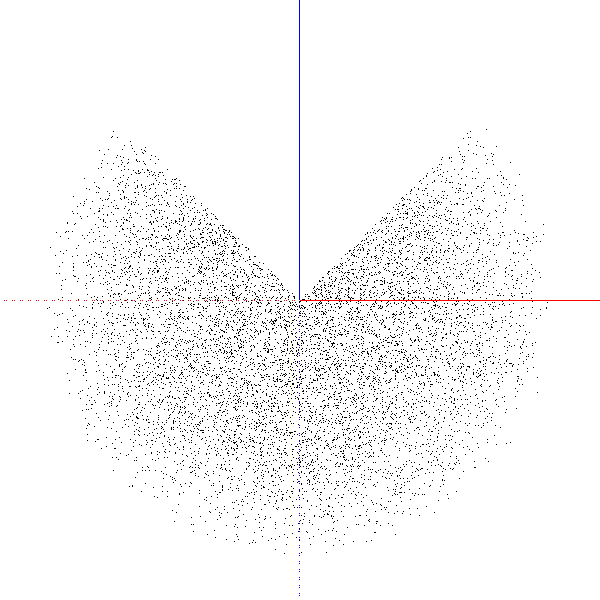
\includegraphics[width=178pt]{goal_list_top} 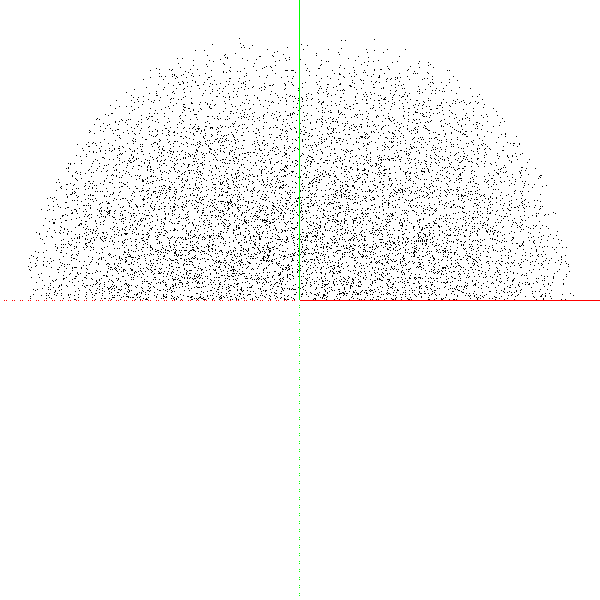
\includegraphics[width=178pt]{goal_list_front}
        \caption{Liste de buts théoriquement atteignables}
        \label{fig:goal_list}
    \end{figure}
    
    \item[$\bullet$] La deuxième contient les observations faites après utilisation de la bibliothèque Ikpy qui contient un modèle inverse. Cette liste ne contient que des observations, donc des point qui sont réellement atteignable. Avec ce modèle inverse il est possible de comparer l'efficacité d'un modèle inverse existant, ici Ikpy, avec le modèle inverse généré par les algorithmes.
\end{itemize}

\section{Paramètres}

Il existe plusieurs paramètres aux différents algorithmes utilisés. Afin de pouvoir les comparer, il faut d'abord trouver les paramètres les plus optimisés pour chacune des instances. L'apprentissage se résume à remplir de la manière la plus efficace possible un catalogue qui représente la vie d'un robot. Un paramètre commun à tous ces apprentissage est donc la taille du catalogue. On peut facilement imaginer qu'un catalogue plus grand permet d'avoir une meilleure précision et une meilleure couverture de l'espace. Deux valeurs de ce paramètre ont étées testées pour ne pas avoir un nombre trop important de version à tester. Afin de vérifier l'hypothèses, ces deux paramètres sont 1 000 entrées dans le catalogue pour représenter une borne inférieure, ainsi que 100 000 entrées dans le catalogue.

\subsection{Motor Babling}

\`A chaque étape du Motor Babling, une posture est choisie en donnant un angle aléatoire à chacun des moteurs généré uniformément sur leur portée. C'est une exploration de tout l'espace moteur du robot, donc tout point atteignable par ce robot possède donc une probabilité non nul d'être dans le catalogue. J'en déduis que la couverture du Motor Babling augmente avec la taille de son catalogue.

Plus il y a de points dans ce catalogue, la distance entre un but et les points du catalogue utilisés dans l'interpolation sera petite, donc la précision de l'algorithme augmente aussi avec la taille de son catalogue.

\subsection{Goal Babling}

Quelque soit l'algorithme de génération du but, pour initier le Goal Babling il faut exécuter un certain nombre d'étape de Motor Babling. C'est donc un paramètre à prendre en compte. Comme il faut commencer par un certain nombre d'étapes de Motor Babling, la borne inférieure testée pour ce paramètre est une proportion de 0.01 étapes sur le nombre total d'entrée du catalogue. Si la proportion est trop grande, cela reviens à faire simplement du Motor Babling. La deuxième valeur testée pour ce paramètre sera donc une proportion de 0.2 sur le nombre total d'entrée du catalogue.

Lorsqu'un but est choisi, une nouvelle entrée dans le catalogue est crée à partir d'une perturbation de donnée existante. Cette perturbation est un autre paramètre à prendre en compte pour du Goal Babling. Avec une perturbation plus elevée, la posture générée sera normalement plus loin de la posture selectionnée. La couverture d'un algorithme augmente donc avec la perturbation. Cependant, l'observation de la posture générée a plus de chance d'être distante du but demandé, et donc la perturbation peut déteriorer la précision de l'algorithme. Les valeurs utilisées pour ce paramètre sont une proportion de 0.05 de la portée du moteur, ainsi qu'une proportion de 0.2 de la portée du moteur.

\subsection{Agnostric Goal Generation}

La génération de but agnostique utilise une zone qui est calculée à partir de la zone couverte par les observations du catalogue. Afin d'ajouter un taux d'exploration à l'algorithme, la zone de génération des buts sera une extension de la zone couverte par le catalogue. Plus le coefficient d'extension est grand, plus la zone dans laquelle les buts sont générés sera grande. Plus le coefficient est grand, plus la zone de génération de but est grande, or le nombre d'entrée du catalogue ne change pas. Ce coefficient impacte donc positivement la couverture mais négativement la précision. Deux valeurs sont utilisées pour ce paramètre. La première est de 0.7, une borne inférieur qui permet d'illustrer si un autre paramètre impacte plus l'exploration que celui-ci. La deuxième est 1.4, valeur supposée non extrême: une valeur trop grande donne une génération de but impossible à atteindre. Le robot se forcerait à n'atteindre que les extrémités de son espace de travail.

\subsection{Frontier Goal Generation}

Lors de l'utilisation du Frontier Goal Generator, ou plus largement du Goals on Grid, il existe un coefficient d'exploration p. Avec une probabilité p l'algorithme va choisir d'explorer l'espace, et avec une probabilité p-1, l'alogirthme choisi d'exploiter le catalogue. Trois valeurs de p ont étées testées. Les dornes 0.01 et 0.9, ainsi qu'une valeur intermédiaire 0.5.

Il est aussi possible de changer la taille d'une cellule pour l'utilisation de Goals on Grid. Une taille de cellule plus petite représentera plus présicemment la zone atteinte par le catalogue, mais rendra l'exploration de l'espace plus lente. Une taille de cellule trop grande et l'algorithme devient une simple génération agnostique. J'ai choisi de fixer la taille de l'espace, et je détermine la taille d'une cellule à partir d'un certain nombre de division de cet espace. Deux valeurs pour ce paramètre ont été testée: 10 divisions (ce qui reviens à des cellules de tailles de 10cm³), et 1 000 divisions (ce qui reviens à des cellules de 1mm³).

%%%%%%%%%%%%%%%%%%%
% % % SECTION % % %
%%%%%%%%%%%%%%%%%%%
% les conclusions
\chapter{Conclusion}


\end{document}
